\section{Introduction}

In previous chapters I have advocated the use of machine learning for
autotuning. In this chapter, I present OmniTune, a framework for
extensible, distributed autotuning using machine learning. OmniTune
provides a replacement for the kinds of ad-hoc tuning typically
performed by expert programmers by providing runtime prediction of
tunable parameters using collaborative, online learning of
optimisation spaces. First I describe the high level overview of the
approach to autotuning, then I describe the system architecture and
set of interfaces exposed by Omnitune.


\section{Predicting Optimisation Parameter Values}

\begin{figure}[b]
\centering
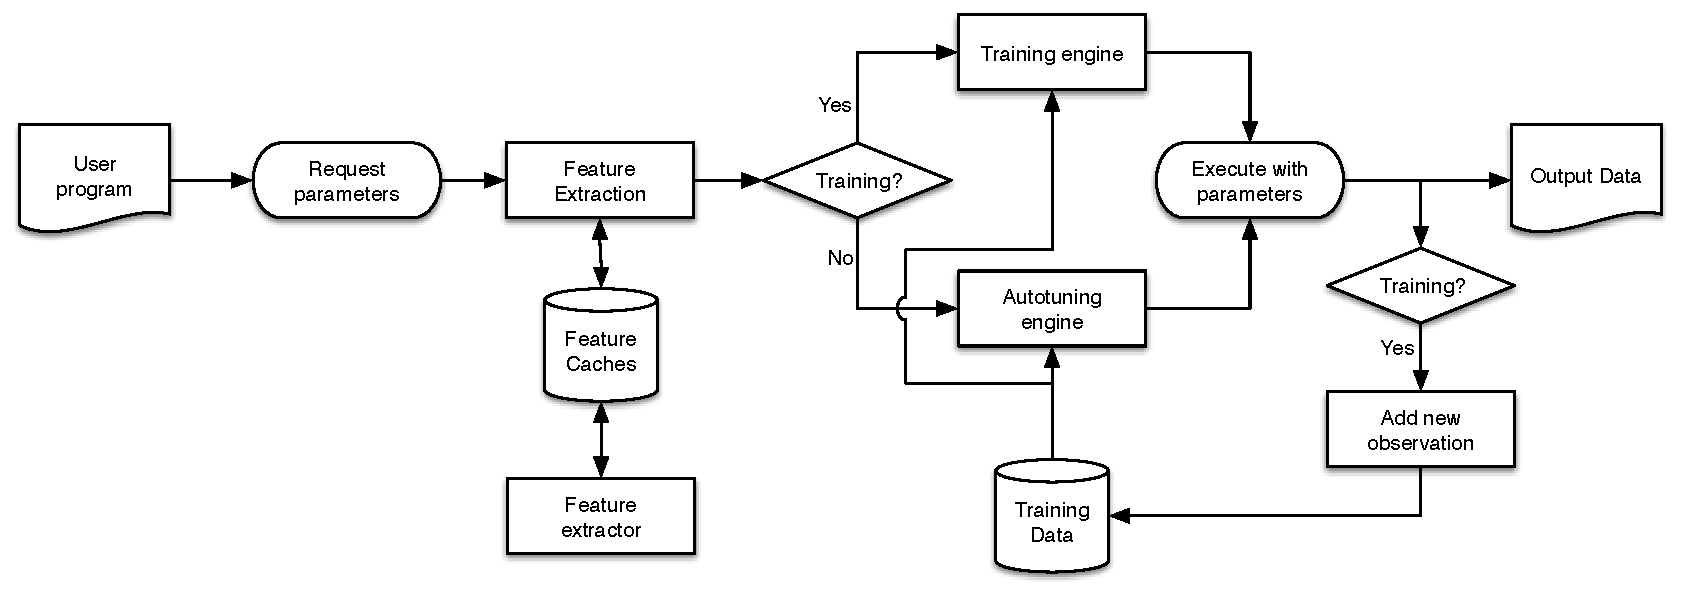
\includegraphics[width=\textwidth]{img/omnitune-system-flow.pdf}
\caption[Optimisation parameter selection with OmniTune]{%
  The process of selecting optimisation parameter values for a given
  user program with OmniTune.%
}
\label{fig:omnitune-system-flow}
\end{figure}

The goal of machine learning-enabled autotuning is to \emph{predict}
the values for optimisation parameters to maximise some measure of
profit. These predictions are based on models built from prior
observations. The prediction quality is influenced by the number of
prior observations. OmniTune supports both prediction of parameters
based on prior observations, and a method for collecting these
observations. When a client program requests parameter values, it
indicates whether the request is for training or performance purposes,
and uses a different backend to select parameter values for each. New
observations can then be added once parameters have been evaluated.
Figure~\ref{fig:omnitune-system-flow} shows this process.


\section{System Architecture and Interface}

\begin{figure}
\centering
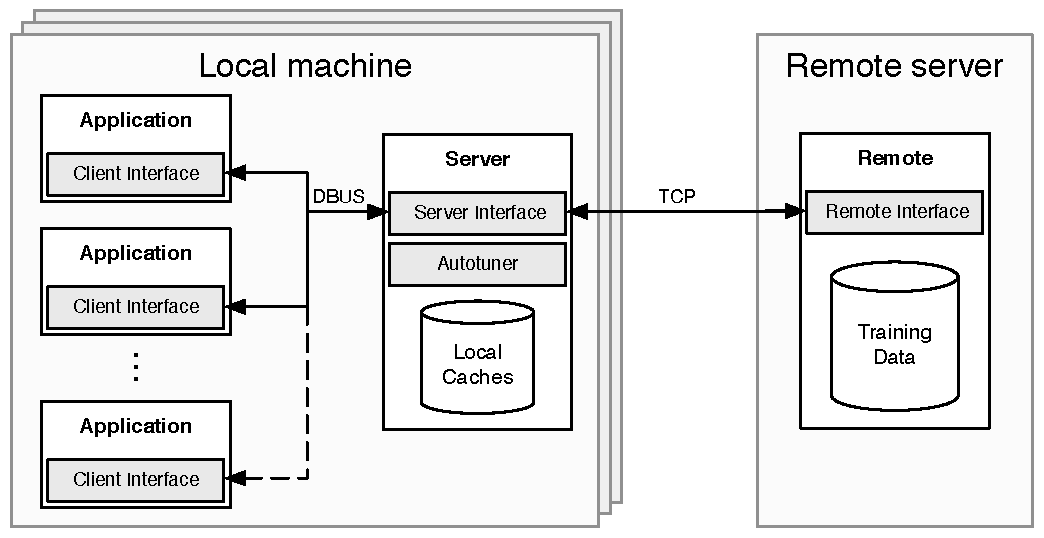
\includegraphics[width=.9\textwidth]{img/omnitune-system-overview.pdf}
\caption[OmniTune system diagram]{%
  High level overview of OmniTune components.%
}
\label{fig:omnitune-system-overview}
\end{figure}

Common implementations of autotuning in the literature either: embed
the autotuning logic within the each target application, or take a
standalone approach in which the autotuner is a program which must be
invoked by the user to tune a target application. Embedding the
autotuner within each target application has the advantage of
providing ``always-on'' behaviour, but is infeasible for complex
systems in which the cost of building machine learning models must be
added to each program run. The standalone approach separates the
autotuning logic, at the expense of adding one additional step to the
build process. The approach taken in OmniTune aims to capture the
advantages of both techniques by implementing a autotuning \emph{as a
  service}, with only the lightweight communication logic embedded in
the target applications.

Omnitune is built around a three tier client-server model. The
applications which are to be autotuned are the \emph{clients}. These
clients commmunicate with a system-wide \emph{server}, which handles
autotuning requests. The server communicates and caches data sourced
from a \emph{remote}, which maintains a global store of all autotuning
data. Figure~\ref{fig:omnitune-system-overview} shows this structure.

There is a many to one relationship between clients, servers, and
remotes, such that a single remote may handle connections to multiple
servers, which in turn may accept connections from multiple
clients. This design has two primary advantages: the first is that it
decouples the autotuning logic from that of the client program,
allowing developers to easily repurpose the autotuning framework to
target additional optimisation parameters without a significant
development overhead for the target applications; the second advantage
is that this enables collective tuning, in which training data
gathered from a range of devices can be accessed and added to by any
OmniTune server.

OmniTune supports autotuning using a separate offline training phase,
online training, or a mixture of both. Figure~\ref{fig:omnitune-comms}
shows an example pattern of communication between the three tiers of
an OmniTune system, showing a distinct training phase. Note that this
training phase is enforced only by the client. The following sections
describe the interfaces between the three components.


\begin{figure}[b]
\centering
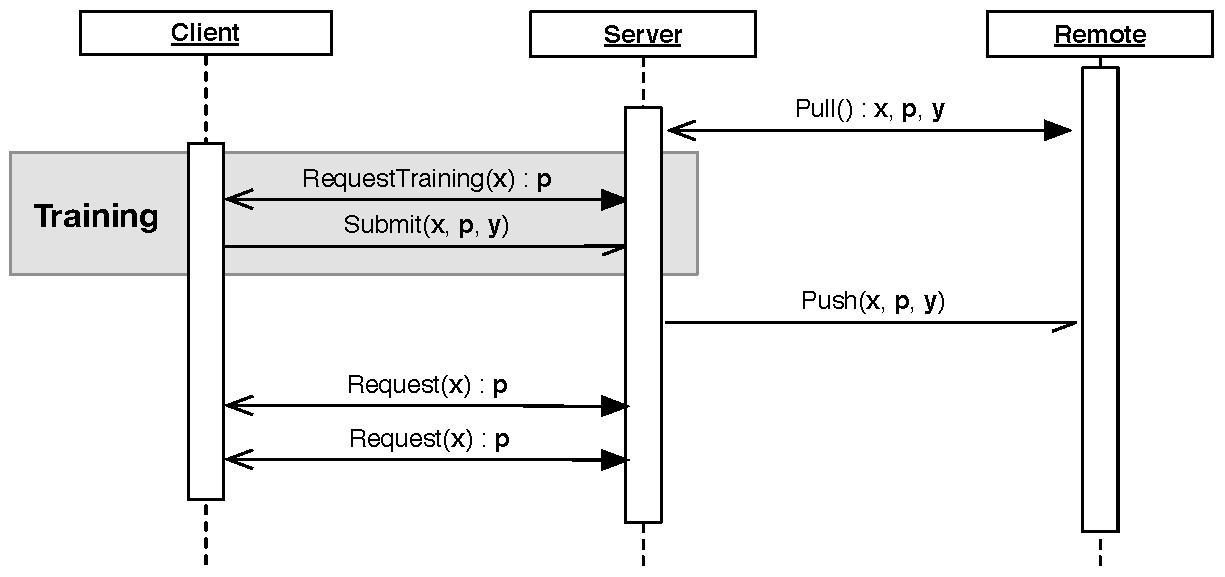
\includegraphics[width=.7\textwidth]{img/omnitune-comms}
\caption[Communication pattern between OmniTune components]{%
  An example communication pattern between OmniTune components,
  showing an offline training phase.%
}
\label{fig:omnitune-comms}
\end{figure}


\subsection{Client Interface: Lightweight Communication}

Client applications communicate with an OmniTune server through four
operations:
%
\begin{itemize}
\item \textsc{Request}$(x) \to p$ Given a set of explanatory variables
  $x$, request a set of parameter values $p$ to maximise performance.
\item \textsc{RequestTraining}$(x) \to p$ Given a set of explanatory
  variables $x$, allow the server to select a set of parameter values
  $p$ for evaluating their fitness.
\item \textsc{Submit}$(x, p, y)$ Submit an observed measurement of
  fitness $y$ of parameters $p$, given explantory variables $x$.
\item \textsc{Refuse}$(x, p)$ Refuse a set of parameters $p$ given a
  set of explanatory variables $x$. Once refused, those parameters
  will not be returned by any subsequent calls to \textsc{Request()}
  or \textsc{RequestTraining()}.
\end{itemize}
%
This set of operations enables the core functionality of an autotuner,
while providing flexibility for the client to control how and when
training data is collected.


\subsection{Server: Autotuning Engine}

For each autotuning-capable machine, a system-level daemon hosts a
DBus session bus which client processes communicate with. This daemon
acts as an intermediate between the training data and the client
applications, \emph{serving} requests for optimisation parameter
values. Servers operations are application-specific, so there is a set
of operations to implement autotuning of each supported optimisation
target.

The server is implemented as a standalone Python program, and contains
a library of machine learning tools to perform parameter prediction,
interfacing with Weka using the JNI. Weka is a suite of data mining
software developed by the University of Waikato, freely available
under the GNU GPL
license~\footnote{http://www.cs.waikato.ac.nz/ml/weka/}. OmniTune
servers may perform additional feature extraction of explanatory
variables supplied by incoming client requests. The reason for
performing feature extraction on the server as opposed to on the
client side is that this allows the results of expensive operations
(for example, analysing source code of target applications) to be
cached for use across the lifespan of client applications. The
contents of these local caches are periodically and asynchronously
synced with the remote, to maintain a global store of lookup tables
for expensive operations.

On launch, the server requests the latest training data from the
remote, which it uses to build the relevant models for performing
prediction of optimisation parameter values. Servers communicate with
remotes by submitting or requesting training data in batches, using
two operations:
%
\begin{itemize}
\item \textsc{Push}$(\bf{f}, \bf{c})$ Submit a set of labelled training
  points as pairs $(f,c)$.
\item \textsc{Pull}$() \to (\bf{f}, \bf{c})$ Request training data as a
  set of labelled $(f,c)$ pairs.
\end{itemize}


\subsection{Remote: Distributed Training Data}

The role of the remote is to provide bookkeeping of training data for
machine learning. Using the interface described in the previous
section, remotes allow shared access to data from multiple servers
using a transactional communication pattern.


\section{Summary}

This chapter has described the architecture of of OmniTune, a
distributed autotuner which is capable of performing runtime
prediction of optimal workgroup sizes using a variety of machine
learning approaches. OmniTune uses a client-server model to decouple
the autotuning logic from target programs and to maintain separation
of concerns. It uses lightweight inter-process communication to
achieve low latency autotuning, and uses caches and lookup tables to
minimise the one-off costs of feature extraction.
